%%
%%                  TEMPLATE for Math 436 project report
%%
\documentclass[11pt]{amsart}
%%% WARNING: Do NOT change the page size, fonts, or margins!  Penalties will apply.

% \usepackage{chemformula}
\usepackage[version=4]{mhchem}  % Used for chemical equations
\usepackage{graphicx}
\usepackage{amssymb,amsmath,amsthm}
\usepackage{placeins} %enables \FloatBarrier, which prevents figures and tables from going below it.
\usepackage{hyperref} %makes cross references into hyperlinks. 
\graphicspath{ {./images/} }

\begin{document}

\title{Go With the Flow: Optimal Sailboat Racing}
\author{Connor McBride, Ethan Palenske, Jackson Pond}

% Change the date to match the date you actually wrote this paper
\date{\today} % or use \today

\begin{abstract}
In this paper we will try to model the optimal path in the historical M\&M 100 Miler sailing race. Many forces impact optimal sailing, including wind direction, current, and waves, making this a challenging problem to model accurately. The primary questions we work to answer are what the simplest model is that rediscovers real sailing techniques, such as tacking, and how many parameters we can add into our model while still being able to solve it and get reasonable results. We solve the classic Zermelo Navigation Problem assuming constant boat velocity and fixed current drift vector field. Further iterations involve relying on wind instead of a motor, taking into account the impact of the islands on wind and current speed, and adding land penalties. Our more accurate models were able to find a path that matched the speeds of real-world sailors from the year we got current and wind data.

\end{abstract}

\maketitle % this actually makes the title

%% First Section
\section{Background}

% BACKGROUND ABOUT THE RACE HERE
\par The historic M\&M 100 Miler sailing race takes place annually in Lake Michigan, and despite its name, is about $42$ nautical miles in length \cite{mmyc2024charts}. While this is a family-centered race with no prizes or larger impact, the problem of optimizing sailing routes is an ancient one, and one that is growing in importance today.

\begin{figure}[htbp]
    \centering
    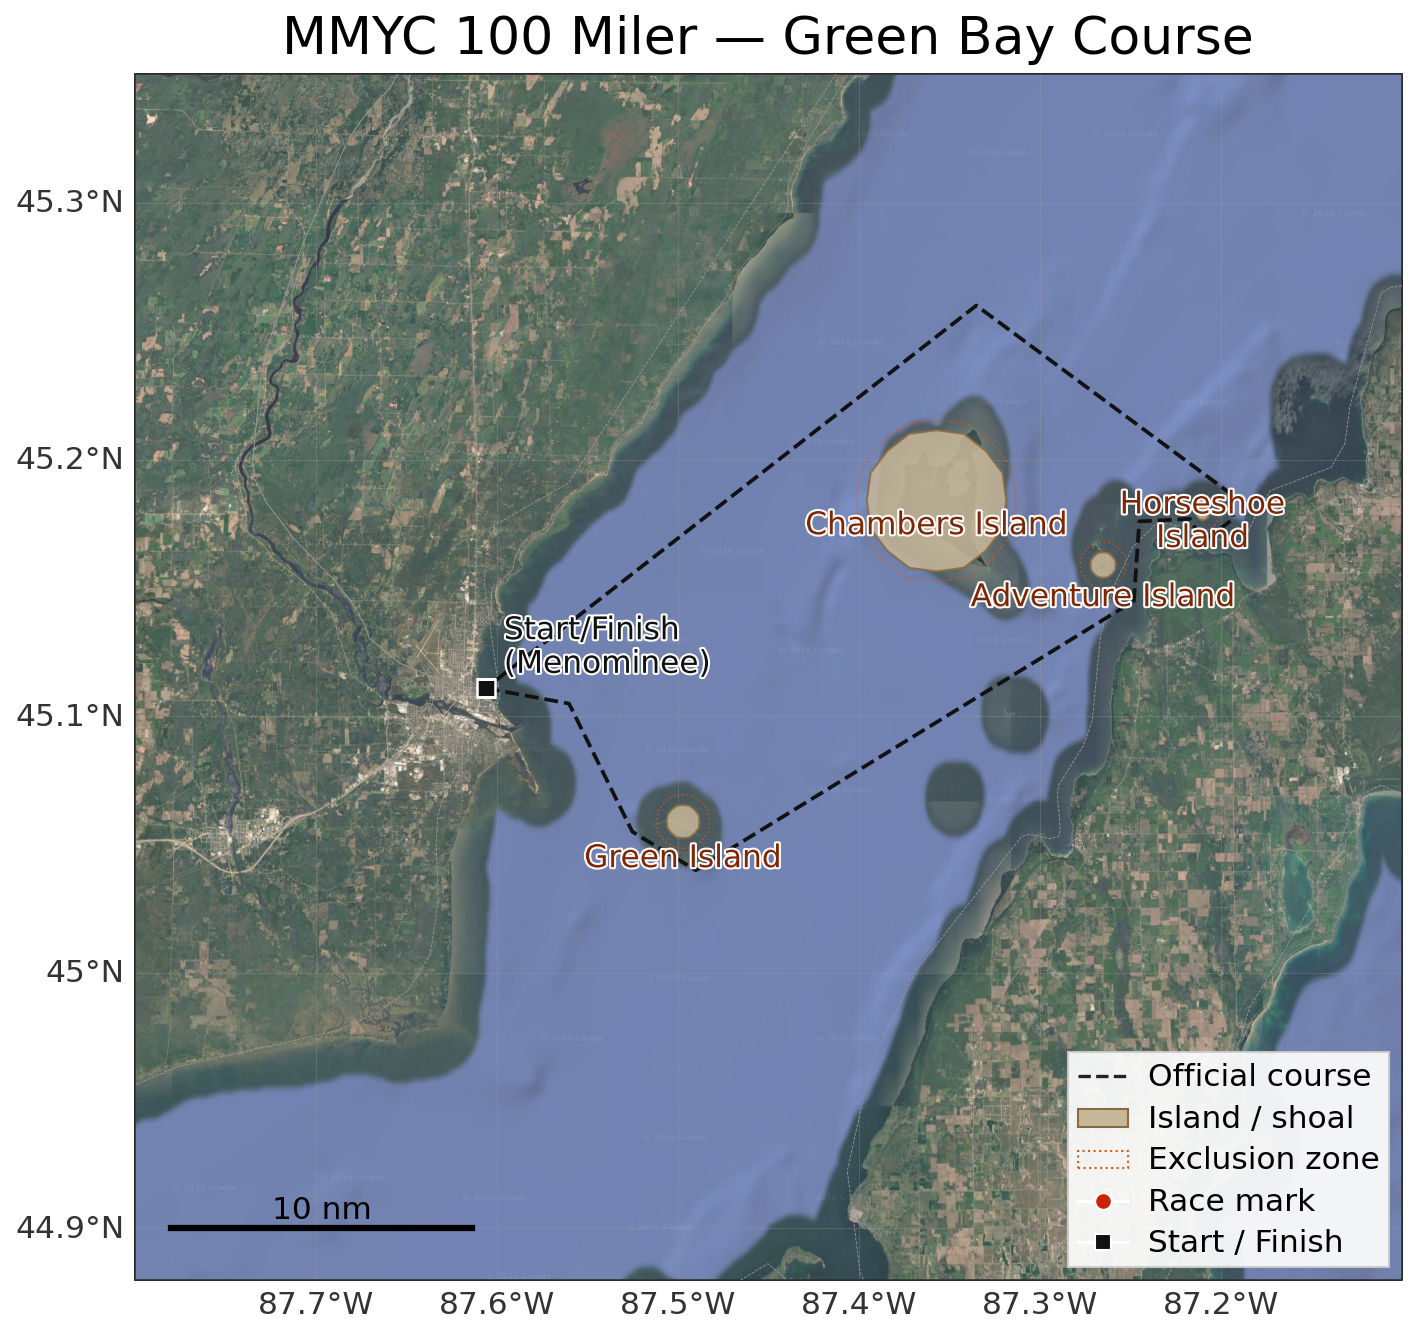
\includegraphics[width=0.5\textwidth]{images/100miler_race.png}
    \caption{The M\&M 100 Miler race course.}
    \label{fig:100milder_map}
\end{figure}

\par Triangular sails were first used in the 2nd century, and since then, determining optimal routes for boats has been a key question not just for racing, but also for commerce, avoiding pirates, and catching commercial vessels that are avoiding you. Now that cargo vessels are beginning to explore adding sails to make their travel more efficient, optimal sailing routes for commerce are a key issue in global supply chain \cite{page2026vela}.

\par In this project we work to solve a related problem by modeling the optimal route for the 100 Miler race. We started from the simplest case and then increased the model complexity from there.

\par The primary question this paper seeks to determine is what the simplest model is that re-discovers real world sailing techniques, particularly tacking and jibing. Similarly, we wanted to determine the most physically realistic model we could put together that could still be solved numerically and yield realistic results. Our code is available on our GitHub repository \cite{repo_2026}.

%% Second Section 
\section{Mathematical Representations}

\par In this section we go over the models we used to represent sailing dynamics.

% Talk about square sails vs. triangular sails

\subsection*{Model 1: Zermelo Navigation Problem}

\par We first solved the classical Zermelo Navigation Problem, which involves directing a motorboat moving at constant speed $v$ through a body of water with a variable current, given by the vector field $\vec{w}.$ The problem is to determine the path that minimizes the time it takes to get between two fixed points. In this case the control is the angle between the boat's hedding and the $x$-axis, $\theta.$

\par Our state $\vec{s}$ is given by $$ \begin{bmatrix} x \\ y \end{bmatrix}$$ which are simply our $x$ and $y$ coordinates. 

The control vector, or $\vec{u}$, is given by the $x$ and $y$ components of the fixed velocity $v$ in the direction of $\theta,$ or

$$ \begin{bmatrix} u_1 \\ u_2 \end{bmatrix} = v \begin{bmatrix} \cos(\theta) \\ \sin(\theta) \end{bmatrix}.$$

The velocity vector is the control vector plus the effects of the drift $\vec w$:

$$ \dot{\begin{bmatrix} x \\ y \end{bmatrix}} = v \begin{bmatrix} \cos(\theta) \\ \sin(\theta) \end{bmatrix} + \begin{bmatrix} w_1(x, y) \\ w_2(x, y) \end{bmatrix}$$

This problem's constraints are fixed endpoints and a norm for our control $u$:
$$ \| u \| = v, \;\; \vec{s}(t_0) = \vec{s}_0, \;\; \vec{s}(t_f) = \vec{s}_f.$$

Thus, our functional to be minimized is
\begin{align*}
    J[u] &= \int_{t_0}^{t_f} 1 dt\\
    \text{subject to } \dot{\vec{s}} &= \vec{u}(t) + \vec{w}(\vec{s}(t)),\\
    \vec{s}(t_0) &= \vec{s}_0,\\
    \vec{s}(t_f) &= \vec{s}_f,\\
    \text{and } \| u \| &= v.
\end{align*}

\subsection*{Model 2: Square-Sail Dynamics}

\par The next approach used simple sailing dynamics modeled on square-sailed boats. The assumption is the boat moves in the same direction as the sail is facing, with speed proportional to the exposure of the sail to the wind. The dynamics are very similar to the previous problem, with the angle of the boat from the $x$-axis, $\theta,$ being our control, and $\phi$ being the angle of the wind in relation to the $x$-axis. The primary differences between this model and the previous one is that we no longer have the constraint of constant speed and the dynamics are slightly different:

$$ \begin{bmatrix} u_1 \\ u_2 \end{bmatrix} = v \begin{bmatrix} \cos(\theta - \phi) \cos(\theta) \\ \cos(\theta - \phi) \sin(\theta) \end{bmatrix}.$$

and the constraint $\| u \| = v$ becomes $\| u \| = v |\cos(\theta - \phi)|.$ Intuitively the $\cos(\theta - \phi)$ is the dot product between the boat's heading and the wind's direction, dictating the exposure of the sail to the wind. The rest of the setup, including the functional, are identical to the previous one.

\subsection*{Model 3: Triangular-Sail Dynamics}

\par However, boats with triangular sails work very differently from boats with square sails. Instead of being pushed by the wind, triangular sails act similar to airplane wings: the wind blows faster over their front than their back, causing a pressure differential that \textit{pulls} the boat in the direction the sail is facing. This means that boats can sail nearly upwind, but also makes sailing directly downwind very unstable.

\subsection*{Model 4: Acceleration and Land Penalties}

\par Each of the previous models assumed that wind and current directly impacted a boat's velocity. However, it is more accurate to model these as changing the boat's \textit{acceleration} instead.

%% Third Section
\section{Solutions}

\par In this section we solve the optimal control problems from the previous section and explain the numerical methods we used to compute optimal paths.

\subsection*{Model 1: Zermelo Navigation Problem}


\subsection*{Model 2: Square-Sail Dynamics}


\subsection*{Model 3: Triangular-Sail Dynamics}


\subsection*{Model 4: Acceleration and Land Penalties}

%%Fourth Section
\section{Interpretation}


\subsection*{Appropriateness of models}


\subsection*{Potential improvements}

\par While we accounted for the impact of current, we did not account for the impact of waves on sailing.

\subsection*{Impact}
% The impact of our results / this problem

\par With continually growing concerns about the impact of fossil fuel use on the environment, and with the ever-present motivation to cut costs, the impact of cutting shipping emissions using sails cannot be overstated. One company, Vela, is already using a 100\% wind-powered ship with triangular sails to transport cargo across the ocean faster than other shipping vessels. Not only does the prototype, a type of trimarian, cut down on emissions, it also is much quieter, less disturbing to wildlife than traditional shipping, and individual boats can cross the Atlantic 2-4 times faster than traditional cargo ships \cite{page2026vela}.

\par As this technology grows more widespread, the problem of determining optimal sailing routes will once more be extremely important to global commerce, making markets more efficient and helping to combat global climate change.

%%Fifth Section
\section{Conclusion}

\par While the simplest two models we worked with were not able to rediscover real sailing techniques, the more complicated ones were.

%%FERPA Release
\section{FERPA Release}
We give Dr. Jarvis and other instructors at BYU teaching ACME classes permission to share our project as an example of a good project in future classes they teach.

\begin{itemize}
    \item Connor McBride
    \item Ethan Palenske
    \item Jackson Pond
\end{itemize}

%%%%%%%%%%%%%%%%%%%%%%%%%%%%%%%%%%%%%
%% Bibliography below
%%%%%%%%%%%%%%%%%%%%%%%%%%%%%%%%%%%%%
\FloatBarrier % Keep the figures from being put after the bibliography
\newpage
\bibliography{refs}
\bibliographystyle{alpha}

\end{document}
